\documentclass[a4paper]{article}

%image
\usepackage{graphicx}

%Chinese
\usepackage[encapsulated]{CJK}
\usepackage{ucs}
\usepackage[utf8x]{inputenc}
\setlength{\parindent}{0em}
\setlength{\parskip}{0.5em}
\renewcommand{\contentsname}{目录}
\renewcommand{\figurename}{图}
\renewcommand{\tablename}{表}

%code
\usepackage{listings}

%table
% \usepackage{longtable}
% \usepackage{multirow}

% \usepackage[colorlinks,linkcolor=red]{hyperref}
\newcounter{rowno}
\title{
    Java Script Interpretor - StairJS\\
    \small{--Not a Toy!}
}
\author{
    李其迈\\
    计算机科学与技术学院\\
    浙江大学\\
    \and 
    海杰文\\
    计算机科学与技术学院\\
    浙江大学\\
    \and 
    陈广翔\\
    计算机科学与技术学院\\
    浙江大学\\
    \and 
    蔡武威\\
    计算机科学与技术学院\\
    浙江大学\\
}

\pdfinfo{%
  /Title    (Java Script Interpretor - StairJS)
  /Author   (LiQimai HaiJieWen ChenGuangxiang CaiWuwei)
  /Creator  ()
  /Producer ()
  /Subject  ()
  /Keywords ()
}

\begin{document}
\begin{CJK}{UTF8}{gbsn}
% \maketitle
\begin{titlepage}
    \clearpage
    %% temporary titles
    % command to provide stretchy vertical space in proportion
    \newcommand\nbvspace[1][3]{\vspace*{\stretch{#1}}}
    % allow some slack to avoid under/overfull boxes
    \newcommand\nbstretchyspace{\spaceskip0.5em plus 0.25em minus 0.25em}
    % To improve spacing on titlepages
    \newcommand{\nbtitlestretch}{\spaceskip0.6em}
    \pagestyle{empty}
    \begin{center}
        \bfseries
        \nbvspace[3]
        \normalsize
        DOCUMENT\\
        OF\\
        \Huge
        {\nbtitlestretch\huge Stair JavaScript}

        % \nbvspace[1]
        \normalsize

        Another Java Script Interpreter\\
        \nbvspace[1]
        \small 
        THIS\\
        IS\\
        MORE THAN A TOY\\[0.5em]
        % \footnotesize AUTHOR OF ``A WORKING ALGEBRA,'' ``WIRELESS TELEGRAPHY,\\
        % ITS HISTORY, THEORY AND PRACTICE,'' ETC., ETC.

        \nbvspace[2]

        % 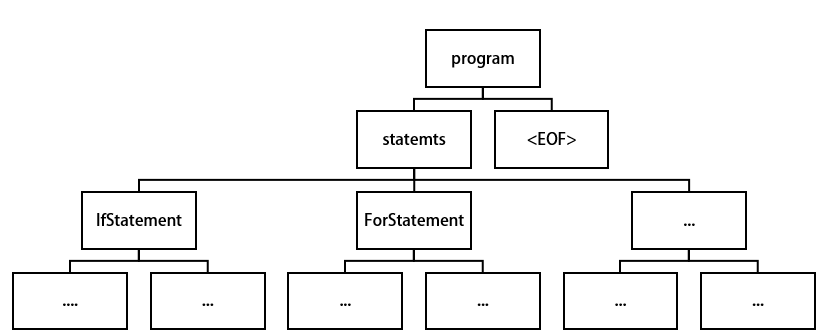
\includegraphics[width=1.5in]{pictures/AST.eps}
        \nbvspace[3]
        \normalsize

        BY\\
        \large
        李其迈 海杰文 陈广翔 蔡武威
        \nbvspace[1]
    \end{center}
\end{titlepage}

\newpage

\tableofcontents
\newpage
\section{概述}
    StairJS是用python3实现的一个较为完善的JavaScript解释器,支持了JavaScript大部分基本特性。其所能够解释的语言是JavaScipt的一个子集。StairJS实现了以下特性:
    % \begin{list}{-}
    \setcounter{rowno}{0}
    \begin{list}{\therowno.}{\usecounter{rowno}\setlength{\rightmargin}{\leftmargin}}
        \item 两种模式:文件解释模式、交互式模式 
        \item 支持JavaScript中所有的基本类型 
        \item 几乎所有运算符 
        \item 13级运算优先级 
        \item 大部分语句 
        \item 函数的定义、调用、递归以及成员函数和高阶函数 
        \item 面向对象 
        \item 垃圾回收机制 
        \item 注释 
        \item 错误提示信息
    \end{list}
\section{如何使用StairJS}
    \subsection{第一个程序Hello World}
        运行StairJS,你需要:
        \setcounter{rowno}{0}
        \begin{list}{\therowno.}{\usecounter{rowno}\setlength{\rightmargin}{\leftmargin}}
            \item Python3的解释器
            \item PLY库
        \end{list}
        因为 StairJS 是用 Python3 开发的,所以首先确保你有一个Python3的解释器。StairJS 在 Python3.4.3下做过完整的测试,保证可以运行。 Python3 版本之间差异不大,应该都可以成功运行 StairJS 。有了 python 解释器后,还需要安装 PLY-3.8 这个 python 的库。访问 PLY-3.8 的官网 {\tt http://www.dabeaz.com/ply/} ,下载并安装后即可运行我们的 StairJS 。\\

        \hangafter 1
        \hangindent 4em
        不给任何参数运行 StairJS.py ,会进入交互式模式,并显示版本号。\\
        {\tt 
            root@desktop: python StairJS.py\\
            Stair JavaScript Interpreter V1.0\\
            Powered by Li Qimai, Hai Jiewen, Chen Guangxiang, Cai Wuwei\\
            >>>\\
        }

        \hangafter 6
        \hangindent 4em
        \verb1">>>"1是输入提示符,表示解释器正在等待输入代码。让我们输入{\tt print 'Hello World'},并按enter键。此时显示"...",提示等待后续输入, 我们直接回车输入一个空行, 就可以看到程序显示了 {\tt Hello World} 。 用户可以一次输入多行,StairJS会一直读入代码,直到遇到空行为止,之后将会开始解释执行刚才的输入。 {\tt print} 语句\footnote{详见 \S\ref{statment} 中的 {\tt print} 语句。}是我们额外添加的一个关键字,提供一种输出的手段。程序执行结果如下:\\
        {\tt
            >>>print 'Hello World'\\
            ...\\
            Hello World\\
            >>>\\
        }

        \hangafter 1
        \hangindent 4em
        之后输入{\tt exit}退出解释器,回到终端。\\
        {\tt
            >>>exit\\
            Bye!\\
            root@desktop:\\
        }

        \hangafter 1
        \hangindent 4em
        完整的执行过程如下:\\
        {\tt
            root@desktop: python StairJS.py\\
            Stair JavaScript Interpreter V1.0\\
            Powered by Li Qimai, Hai Jiewen, Chen Guangxiang, Cai Wuwei\\
            >>>print 'Hello World'\\
            ...\\
            Hello World\\
            >>>exit\\
            Bye!\\
            root@desktop:\\
        }

    \subsection{两种模式}
        \subsubsection{交互式模式}
            命令:\\
            {\tt python StairJS.py}

            如果不给任何命令行参数,直接运行解释器,即可进入交互式界面。在交互式界面,由用户输入一串以空行结尾的 JavaScript 代码,之后解释器解释这段代码。显示\verb1">>>"1表示正在等待一段全新的代码的输入。显示{\tt"..."}表示正在等待后续输入。

            如果本次输入是一个表达式,则执行完毕后解释器会将表达式的计算结果显示出来。如果本次输入不是表达式,或者是多条表达式,则不会显示结果。

        \subsubsection{文件解释模式}
            \hangafter 1
            \hangindent 4em
            命令:\\
            {\tt python StairJS.py [-i] <JavaScriptSource> <arg>*}

            其中 \verb1<JavaScriptSource>1 是一个JavaScript的源代码文件。\verb1arg1是要传入JavaScript程序的命令行参数。从源代码文件名开始的所有参数将按顺序放入全局变量\verb1args1中。在JavaScript程序中可以通过\verb1args1访问到这些命令行参数。

            编写 JavaScript 程序如下,存入文件{\tt PrintArgs.js}中
            \begin{verbatim}
        /*PrintArgs.js 打印出所有的命令行参数*/
        for(var i in args){
            print i + ":" + args[i]
        }
            \end{verbatim}

            \hangafter 1
            \hangindent 4em
            解释执行{\tt PrintArgs.js},并传入参数{\tt arg1,arg2,arg3},结果如下:\\
            {\tt
                root@desktop: python StairJS.py PrintArgs.js arg1 arg2 arg3\\
                PrintArgs.js \\
                arg1 \\
                arg2 \\
                arg3 \\
            }

            可以在源代码文件前给参数 -i ,则解释器在解释完源代码文件后,会进入交互式界面。此时仍然可以访问文件中定义的变量和各种函数。命令格式如下:\\
            {\tt python StairJS.py -i HelloWorld.js}


\section{StairJS解释流程}
    StairJS 的整个运作过程可以分为两个阶段---语法解析和解释执行。
    \subsection{语法解析}
        除了额外添加的 print 关键字,StairJS 所能够解释执行的语言是 JavaScript 的一个子集。这个子集由\S\ref{BNF}中的 BNF 精确定义。每次拿到JavaScript的源码后, StairJS 会根据 BNF 来做词法分析和语法分析,并建立一棵 AST(Abstract Syntax Tree) 。树中每个叶子节点对应一个终结符,非叶子节点对应于一个非终结符\footnote{这棵树完全符合 Context Free Grammer 的 Parsing Tree 的规范。详细结构见一般的计算理论教材}。AST结构化的描述了输入的JavaScript程序。\\
        \begin{figure}[h]
        \center
        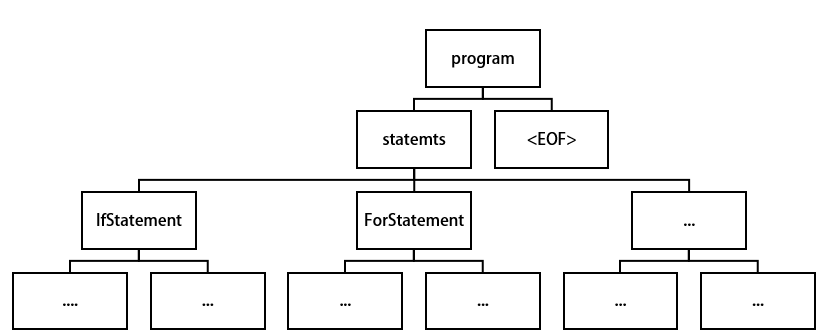
\includegraphics[width=10cm]{pictures/AST.eps}
        \caption{Abstract Syntax Tree示意图}
        \end{figure}

    \subsection{解释执行}
        得到 AST 后,解释器将会遍历 AST 进行解释执行的工作。几乎每个类型的节点都有对应的解释执行该节点的函数。解释某个节点时,只需调用对应函数解释所有的子节点,然后将所有子节点的解释结果综合处理,即可完成该节点的解释工作。整个解释执行的过程其实是一个递归遍历的过程,步骤清晰明了。
\section{基本类型}
    StairJS支持JavaScript的所有基本类型Number, String, Boolean, Object, Function, Null, Undefined。因为解释器是用Python开发的,所以JavaScript的变量最终都要映射成为Python中的变量关系。
    \begin{table}[h]
        \center
        \begin{tabular}{lll}
            JavaScript & Python \\
            \hline
            Number      & int,float \\
            String      & str \\
            Boolean     & bool \\
            Object      & StObject    & 继承自 dict \\
            Function    & StFunction  & 继承自 StObject \\
            Null        & StNULL \\
            Undifined   & StUndifined \\
        \end{tabular}
        \caption{JavaScript变量与Python变量的映射}
    \end{table}

    其中 StObject \footnote{ St 是 StairJS 中 Stair 的简写}是我们定义的一个类,用以表示 JavaScript 中的 Object 。StFunction 是 用来表示 JavaScript 中函数的类。因为在JavaScript中,函数也是对象,所以 StFunction 继承自 StObject 。

    而StNULL和StUndefined虽然是一个类,StNULL和StUndefined在整个解释器中都只有一个实例。

\section{运算符和表达式}
    StairJS 支持除了三目运算符、{\tt delete}、{\tt instanceof}以及前缀的{\tt++}、{\tt--}以外所有的运算符。并且按照 JavaScript 的运算优先级,将所有的运算符分为了14级。具体优先级参见下一页的Table-\ref{OperatorPrecedence}。\\
    其中在StairJS中{\tt==}的效果与{\tt===}一样。\\
    在{\tt"+}运算时,如果有一个操作数是字符串,则会自动将另外一转换成字符串,之后做字符串连接。\\
    函数定义也将被视为一个表达式,可以参与函数调用和取成员、\verb1void typeof1以及相等比较等运算。
    \setcounter{rowno}{0}
    \begin{table}
        \center
        \begin{tabular}{rrp{5cm}c}
            优先级 & 类型 &运算符 & 结合性 \\
            \hline
            \stepcounter{rowno}\therowno & 函数调用和取成员  & \verb1() [] .1              & 从左到右 \\
            \stepcounter{rowno}\therowno & 后缀运算符        & \verb1++ --1                & 从左到右 \\
            \stepcounter{rowno}\therowno & 前缀运算符        & \verb1void typeof + - ~1 !  & 从右到左 \\
            \stepcounter{rowno}\therowno & 乘法类型运算符    & \verb1* / %1                & 从左到右 \\
            \stepcounter{rowno}\therowno & 加法类型运算符    & \verb1+ -1                  & 从左到右 \\
            \stepcounter{rowno}\therowno & 移位运算符        & \verb1<< >> >>>1            & 从左到右 \\
            \stepcounter{rowno}\therowno & 关系运算符        & \verb1< > <= >=1            & 从左到右 \\
            \stepcounter{rowno}\therowno & 等于运算符        & \verb1== != === !==1        & 从左到右 \\
            \stepcounter{rowno}\therowno & 按位与            & \verb1&1                    & 从左到右 \\
            \stepcounter{rowno}\therowno & 按位异或          & \verb1^1                    & 从左到右 \\
            \stepcounter{rowno}\therowno & 按位或            & \verb1|1                    & 从左到右 \\
            \stepcounter{rowno}\therowno & 逻辑与            & \verb1&&1                   & 从左到右 \\
            \stepcounter{rowno}\therowno & 逻辑或            & \verb1||1                   & 从左到右 \\
            \stepcounter{rowno}\therowno & 赋值              & \verb1= *= /= %= += -= <<=1 \verb1>>= >>>= &= ^= |=1 & 从右到左 \\
        \end{tabular}
        \caption{运算符优先级}\label{OperatorPrecedence}
    \end{table}

\section{语句}\label{statment}
    支持的语句有:{\tt Empty, Block, Variable Declaration, If, Do-While, While, For, For-Each, Return, Print}
    \subsection{Empty}
        \hangafter 1
        \hangindent 2em
        格式:\\
        {\tt
        ";"\\
        }

        Empty语句为空语句,仅由一个";"组成,什么也不做。有这条语句存在,语句结束可以有多个";",而不影响程序执行。

    \subsection{Block}
        \hangafter 1
        \hangindent 2em
        格式:\\
        {\tt\{ Statement* \}}

        Bloak中可以有零条或多条语句。Block的作用在于可以把多条语句结合成一条语句。

    \subsection{Variable Declaration}
        \hangafter 1
        \hangindent 2em
        格式:\\
        {\tt"var" <Identifier> ("=" Expression)? ";"?}

        变量声明,同时可以用一个表达式来初始化这个变量。


    \subsection{Variable Declaration}
        \hangafter 1
        \hangindent 2em
        格式:\\
        {\tt "if" "(" Expression ")" Statement ("else" Statement)? ";"?}

        if语句,根据Expression的返回值执行不同的语句。如果需要多条语句放在if内,请使用Block语句。

    \subsection{Do-While}
        \hangafter 1
        \hangindent 2em
        格式:\\
        {\tt "do" Statement "while" "(" Expression ")" ";"?}

        重复Statement,直到Expression值为false。

    \subsection{While}
        \hangafter 1
        \hangindent 2em
        格式:\\
        {\tt "while" "(" Expression ")" Statement}

        重复Statement,直到Expression值为false。

    \subsection{For}
        \hangafter 1
        \hangindent 2em
        格式:\\
        {\tt "for" "(" Expression ";" Expression ";" Expression ";" ")" Statement}

        1)第一个Expression在开始时会被执行一次。\\
        2)执行中间的Expression,若返回false则语句执行结束。返回true则执行Statement,然后执行第三个Expression,之后重复2)

    \subsection{For-Each}
        \hangafter 1
        \hangindent 2em
        格式:\\
        {\tt "for" "(" "var" <Identifier> "in" Expression ")" Statement}

        对Expression返回值的所有key值依次赋给变量Identifier,并执行Statement。

    \subsection{Return}
        \hangafter 1
        \hangindent 2em
        格式:\\
        {\tt "return" ( Expression )? ";"?}

        将Expression的值作为返回值从函数中返回。如果没有 Expression ,则返回 undefined 。

    \subsection{Print}
        \hangafter 1
        \hangindent 2em
        格式:\\
        {\tt "print" Expression ";"?}

        将Expression的值打印出来。


\section{函数}
    {\bf 在JavaScript中,函数具有和其它变量相同的地位。函数也是一等公民。} 可以被赋值,可以被传入另外一个函数,也可以从另外一个函数中传回。所以我们定义了一个继承自 StObject\footnote{StObject是表达JavaScript中Object的类}的类StFunction。
    \begin{verbatim}
    class StFunction(StObject):
        def __init__(self):
            super(StFunction, self).__init__()
            self.name = ""
            self.ast = None  # code
            self.argument_list = []
            self.outFunction = None
    \end{verbatim}    
    \begin{description}
        \item[name] 是函数定义时给的名字,在将函数转化为字符串时会使用到。
        \item[ast] 指向该函数的抽象语法树,在调用该函数时会遍历这棵树。
        \item[argument\_list] 函数的参数名字表,传参时需要使用。
        \item[outFunction] 定义该函数的函数的Active Record。
    \end{description}

    \subsection{函数定义}
        函数定义是动态进行的,也就是说,只有当解释器解释到了函数的定义,才会生成这个函数,而未解释到的函数是不存在的。而对于函数内的函数定义,如:\\
        \begin{verbatim}
        function f(){
            function g(a,b){}
            ...
        }
        \end{verbatim}
        每次调用函数f,函数g都会被重新定义一遍。这就是函数的动态定义。

        每次定义函数时,都会生成一个StFunction的实例。之后初始化StFunction的成员变量。比如上面的函数{\tt g},其{\tt name="g"},{\tt ast} 指向g对应的抽象语法树, {argument\_list=["a","b"]}即{\tt g}的参数名称,{\tt outFunction}指向此时{\tt f}的Active Record。

    \subsection{函数调用}
        函数执行之前需要为函数分配一个空间存放它的本地变量。这个存放函数本地变量的空间叫做Active Record(AR)。我们定义类StActiveRecord来表达Active Record。
        \begin{verbatim}
        class StActiveRecord(dict):
            def __init__(self):
                super(StActiveRecord, self).__init__()
                self.return_value = None
                self.this = None
                self.outFunction = None
        \end{verbatim}
        每次调用函数,就会实例化一个StActiveRecord。并根据 StFunction 的 argument\_list 将参数填入 StActiveRecord 中。 outFunction 和 this 同样会被赋值。 outFunction 的详细介绍详见\ref{HighOrderFunction}高阶函数。this的赋值规则见\ref{MemberFunction}成员函数。完成 StActiveRecord 的初始化后,解释器会切换上下文到这个函数的AR,然后遍历这个函数的抽象语法树,解释执行这个函数。

    \subsection{高阶函数}\label{HighOrderFunction}
        {\bf 高阶函数}高阶函数的实现有两个方面,一是函数可以作为参数传入另外一个函数,二是函数可以作为函数返回值,且返回的函数可以访问到定义它的函数的本地变量。接收函数或返回函数的函数,因为它将另外一个函数视为一般的变量,所以被称为高阶函数(High-Order Function)。 

        我们的 StFunction 是继承自 StObject 的,所以这就保证了它可以被当作参数,也可以被当作函数返回值。

        {\bf outFunction}为了让返回的函数可以访问到定义它的函数的本地变量,我们在 StFunction 和 StActiveRecord 中加入了 outFunction 字段。在函数定义时,会把当前正在执行的这个函数的AR赋给 StFunctiond 的 outFunction 。函数调用时,又将StFunction 的 outFunction 赋给 StActiveRecord 的 outFunction。同一个 StFunction 的实例在多次调用时, outFunction 都指向同一个 AR,所以访问的高阶函数的本地变量是相同的 。全局变量也是放在一个AR中的。所以定义在全局的函数的 outFunction 就指向这个全局的AR,也就可以访问全局变量了。我们并没有为全局变量做特殊处理,这符合正交的原则。而全局的AR的 outFunction 值为 None 。

        {\bf 寻找本地变量}用到某一个本地变量时,会先在当前函数的AR里寻找,找不到的话,就在outFunction指向的AR中寻找,并且递归的找下去。这样就实现了函数闭包。

\section{对象}
    我们对面向对象的支持主要体现在this这个关键字上。我们并没有实现基于原型的继承。下面讲解一下StairJS支持哪些与对象有关的语法。
    \subsection{获得对象实例}
        \subsubsection{Object Literal}
            最简单的获得一个对象实例的方法莫过于使用写 JSON 风格的 Object Literal 。
            \begin{verbatim}
            var a = {
                1   : "adf",
                i   : 4*6,
                "f" :   function (){
                            return i
                        },
                3.4 : true
            }
            \end{verbatim}
            JavaScript中的所有对象都是一个字典,对象中存放多条 key-value 项。 其中 number 、 string 和 identifier 可以做 key ,任意表达式\footnote{函数定义是表达式,表达式返回值为函数本身。所以value可以直接是一个函数。}都可以做 value 。JavaScript不区分整数和浮点数,它们都是 number 类型。所以浮点数也可以做 key 。

        \subsubsection{Array Literal}
            除了 Object Literal ,还可以直接写Array Literal。
            \begin{verbatim}
            var a = ['zero','one',,,'four']
            }
            \end{verbatim}
            Array Literal 实质上也是个字典,并不是数组。只不过这个字典所有的key值都是number类型,而且是整数的。上面的写法和下面的写法等价:
            \begin{verbatim}
            var a = {
                0 : 'zero',
                1 : 'one',
                2 : void 0,     \\void 0的值为Undefined
                3 : void 0,
                4 : 'four'
            }
            }
            \end{verbatim}
            在Array Literal中,两个逗号之间可以不指定值,此时默认赋为Undefined。

        \subsubsection{"构造"函数} 
            JavaScript可以通过"构造"函数,制造对象。
            \begin{verbatim}
            function A(){
                this.i = 3
            }
            var a = new A()
            }
            \end{verbatim}
            这就制造出来了一个"A类"对象a。a有一个成员i值为3。其实这个貌似是"构造"函数的函数,并不具有C++/Java里构造函数的特殊地位。详见\S\ref{MemberFunction}成员函数。

    \subsection{成员}
        \subsubsection{访问成员}
            通过运算符{\tt .}和{\tt []}可以访问一个成员。不同的是{\tt "."}后面只可以跟 Identifier, 而{\tt []}中则必须是number或string。
            \begin{verbatim}
            var a = {
                i   : 3
                "j" : 5
            }
            var i = "j"
            a.i     //值为3
            a["j"]  //值为5
            a[i]    //因为i的值为"j",所以和a["j"]等价
            \end{verbatim}
            注意\verb1a[i]1访问到的值由\verb1i1的值决定,不一定是\verb1a.i1。因为i的值为\verb1"j"1,\verb1a[i]1所以和a\verb1["j"]1等价。

        \subsubsection{添加成员}
            JavaScript中随时可以通过赋值语句为对象添加成员。
            \begin{verbatim}
            var a = {}  //获得一个空的object
            a.i = 3
            a[4] = "four"
            a.f = function () {return i}
            }
            \end{verbatim}
            对成员赋值时,如果成员不存在,则会在对象中添加该成员。这就可以很方便的在对象中添加成员变量和成员函数。

    \subsection{成员函数}\label{MemberFunction}
        \subsubsection{this指向哪里?}
            函数的this究竟指向哪里?在StairJS中,一共有三种情况。
            \setcounter{rowno}{0}
            \begin{description}
                \item[\stepcounter{rowno}\therowno. new] 
                {\tt var a = new A()}\\
                此时会实例化一个空的 Object ,并令A中的 this 指向这个 Object 。
                \item[\stepcounter{rowno}\therowno. 作为成员函数] 
                {\tt a.f()}\\
                此时f被视为a的成员函数,毫无疑问f的 this 指向a。
                \item[\stepcounter{rowno}\therowno. 其它情况] 
                如{\tt f()}这样直接调用。\\
                那f的 this 应该和此时 AR 的 this 相同。假如当前 AR 的 this 指向变量 a ,也就是现在的函数被视为 a 的成员函数 ,那么不指明时 f 也应该默认被视为 a 的成员函数。
            \end{description}

        \subsubsection{“构造”函数只是普通函数}
            注意到我们在定义一个函数时,并不需要加入任何特殊的关键字,就可以作为new时需要的函数。也就是说,任何函数都可以被视作构造函数。完全可以写出如下的代码:
            \begin{verbatim}
            var a = {
                f : function (){
                        this.i = 3
                    }
            }
            b = new a.f()   //成员函数作为构造函数
            \end{verbatim}
            {\tt f}这里明显是a的成员函数,但是也可以用来构造对象b。其实new语句,不过是制造出一个空对象,然后令函数f的this指向a,之后运行一遍这个函数而已。上述代码中的\verb1b = new a.f()1和下面的等价:
            \begin{verbatim}
            b = {}
            b.f = a.f
            b.f()
            delete b.f
            \end{verbatim}
            这充分说明了构造函数不具有特殊地位。

\section{BNF}\label{BNF}
    本解释器支持的语言是 JavaScript 的一个子集。精确定义该语言的BNF见 {\tt http://github.com/Nebula1084/StairJS} 中的 {\it BNF for StairScript.html} 。 本文档同目录下也附有一份副本。

\newpage
\end{CJK}
\end{document}

% %hello_world.tex
% \documentclass[a4paper]{article}
% \usepackage{amsmath}
% \usepackage{graphicx}
% \usepackage{subfigure}
% \usepackage{CJKutf8}
% \usepackage{cite}
% \usepackage{array}
% % \usepackage{endnotes}
% \title{
%     Java Script Interpretor - StairJS\\
%     \small{--Not a Toy!}
% }
% \author{
%     \begin{CJK}{UTF8}{gkai}
%         李其迈
%     \end{CJK}
%     \\
%     \begin{CJK}{UTF8}{gkai}
%         学号:3130104246
%     \end{CJK}
%     \and 
%     \begin{CJK}{UTF8}{gkai}
%         海杰文
%     \end{CJK}
%     \\
%     \begin{CJK}{UTF8}{gkai}
%         学号:
%     \end{CJK}
%     \and 
%     \begin{CJK}{UTF8}{gkai}
%         陈广翔
%     \end{CJK}
%     \\
%     \begin{CJK}{UTF8}{gkai}
%         学号:
%     \end{CJK}
%     \and 
%     \begin{CJK}{UTF8}{gkai}
%         蔡武威
%     \end{CJK}
%     \\
%     \begin{CJK}{UTF8}{gkai}
%         学号:
%     \end{CJK}
% }

% \begin{document}
% \maketitle
% \tableofcontents

% \section{section1}
% \section{section2}
% \section{section3}
% \begin{CJK}{UTF8}{gkai}

% %     根目录下包含以下文件:

% %     \begin{tabular}{lp{8cm}}
% %         CalibrationAndBirdeye & 根据输入的文件计算相机内参,之后对各个图片去畸变,变俯视图。\\
% %         image & 文件夹,内有5张测试图片 \\
% %         imagelist.txt & 列有5个测试图片的文件名 \\
% %         report & 实验报告 \\
% %         CalibrationAndBirdeye & 完整的vs工程 \\
% %     \end{tabular} \\ \\ \\
% %     使用方法:\\
% %     \tt{CalibrationAndBirdeye <board\_width> <board\_height> <imagelist>}\\
% %     \begin{center}
% %         \begin{tabular}{lp{8cm}}
% %             board\_width  & 棋盘格每行的角点个数 \\
% %             board\_height & 棋盘格每列的角点个数 \\
% %             imagelist    & 文本文件,存有测试图片名,以空格或回车分开
% %         \end{tabular}
% %     \end{center}

% %     程序会利用imagelist中的所有图片计算相机内参。然后对每张图片,依次显示原图,去畸变后图像和鸟瞰图。

% % \section{运行结果}
% %     利用随程序附带的5张图片进行测试:\\
% %     \hspace{1cm} \tt{CalibrationAndBirdeye 9 6 imagelist.txt} 

% %     % \figurename-\ref{result}为运行结果(见下页)。对比(a)和(b)两张图,可以看出去畸变后,棋盘格的所有边全都变成了直线。而转化成鸟瞰图(c)后,棋盘上每一个格子都变成了正方形。\\
% %     % \begin{figure}
% %     %     \center
% %     %     \subfigure[原图]{\includegraphics[width=5cm]{pictures/origin.eps}}\label{origin}
% %     %     \subfigure[去畸变后]{\includegraphics[width=5cm]{pictures/undistortion.eps}}\label{undistortion}
% %     %     \subfigure[鸟瞰图]{\includegraphics[width=5cm]{pictures/birdeye.eps}}\label{birdeye}
% %     %     \caption{运行结果}\label{result}
% %     % \end{figure}

% % \section{实现方法}
% %     \subsection{棋盘格角点检测}
% %         首先需要找到每一个图片中棋盘格各个角点的位置。调用\\
% %         \begin{tabular}{lll}
% %         \tt{bool findChessboardCorners(}& \tt{InputArray}   & \tt{image, }\\
% %                                         & \tt{Size}         & \tt{patternSize, }\\
% %                                         & \tt{OutputArray}  & \tt{coners, }\\
% %                                         & \tt{int}          & \tt{flags)}
% %         \end{tabular}\\
% %         获得棋盘格角点\tt{coners}。如果没能找到所有的角点,则这张图片废弃。

% %         如果找到了所有的角点,则调用\\
% %         \begin{tabular}{lll}
% %         \tt{void cornerSubPix(} & \tt{InputArray}       & \tt{image,}\\
% %                                 & \tt{InputOutputArray} & \tt{corners,}\\
% %                                 & \tt{Size}             & \tt{winSize,}\\
% %                                 & \tt{Size}             & \tt{zeroZone,}\\
% %                                 & \tt{TermCriteria}     & \tt{criteria)}
% %         \end{tabular}\\
% %         传入\tt{coners}获得更加精确的角点坐标。

% %     \subsection{获得相机内参矩阵和畸变参数}
% %         在之后需要根据角点在像平面的坐标和在物体坐标系下的坐标计算内参。物体坐标系以棋盘格左上角为原点,向右为x轴正方向,向下为y轴正方向,棋盘中小格的变长为单位长度。将像平面的坐标和物体坐标系的坐标准备好,调用函数\\
% %         \begin{tabular}{lll}
% %         \tt{double calibrateCamera(}    & \tt{InputArrayOfArrays}   & \tt{objectPoints,}\\
% %                                         & \tt{InputArrayOfArrays}   & \tt{imagePoints,}\\
% %                                         & \tt{Size}                 & \tt{imageSize,}\\
% %                                         & \tt{InputOutputArray}     & \tt{cameraMatrix,}\\
% %                                         & \tt{InputOutputArray}     & \tt{distCoeffs,}\\
% %                                         & \tt{OutputArrayOfArrays}  & \tt{rvecs,}\\
% %                                         & \tt{OutputArrayOfArrays}  & \tt{tvecs,}\\
% %                                         & \tt{int}                  & \tt{flags,}\\
% %                                         & \tt{TermCriteria}         & \tt{criteria)}
% %         \end{tabular}\\
% %         获得相机内参矩阵\tt{cameraMatrix}和畸变参数\tt{distCoeffs}。

% %     \subsection{图片变换}
% %         现在就可以对我们的图片进行鸟瞰图的转化了。

% %         \subsubsection{去畸变}
% %             首先需要对图像进行去畸变的处理,将内参矩阵和畸变参数传给函数\\
% %             \begin{tabular}{lll}
% %             \tt{void undistort(}    & \tt{InputArray}   & \tt{src,}\\
% %                                     & \tt{OutputArray}  & \tt{dst,}\\
% %                                     & \tt{InputArray}   & \tt{cameraMatrix,}\\
% %                                     & \tt{InputArray}   & \tt{distCoeffs,}\\
% %                                     & \tt{InputArray}   & \tt{newCameraMatrix)}\\
% %             \end{tabular}\\
% %             即可得到无畸变的图像。

% %         \subsubsection{透视变换}
% %             最后需要利用透视变换,将棋盘格在图片中变成矩形。使棋盘格正对这我们,看起来好像俯视图一样。调用函数\\
% %             \begin{tabular}{lll}
% %             \tt{Mat getPerspectiveTransform(}   & \tt{InputArray}   & \tt{src,}\\
% %                                                 & \tt{InputArray}   & \tt{dst)}\\
% %             \end{tabular}\\
% %             获得所需的透视变换矩阵\tt{M}。\\


% %             然后应用这个透视变换。调用函数\\
% %             \begin{tabular}{lll}
% %             \tt{void warpPerspective(}      & \tt{InputArray}   & \tt{src,}\\
% %                                             & \tt{OutputArray}  & \tt{dst,}\\
% %                                             & \tt{InputArray}   & \tt{M,}\\
% %                                             & \tt{Size}         & \tt{dsize,}\\
% %                                             & \tt{int}          & \tt{flags = INTER\_LINEAR)}\\
% %             \end{tabular}\\
% %             其中\tt{flag}一定要有\tt{CV\_WARP\_INVERSE\_MAP}这个参数。因为我们需要进行刚才得到的透视变换的逆变换。输出的\tt{dst}就是我们的最终结果。

% % \section{编程体会}
% %     因为有\it{Learn OpenCV}的源码,这次的作业总体来说比较顺利。主要工作就是把\it{Learn OpenCV}的c源码看懂,之后写一份C++风格的程序就好。但是\it{Learn OpenCV}用的是openCV 2.0的版本,我用的是openCV 3.0所以有许多API都不一样,中间还是费了一番功夫。

% \end{CJK}

% % \begin{thebibliography}{99}
% % \bibitem{Shlens}
% %     Jonathon Shlens,
% %     Google Research,
% %     {\it A Tutorial on Principal Component Analysis},
% %     April 7, 2014, 
% %     Version 3.02.
% % \end{thebibliography}
% % \begin{equation}
% % M_{(x,y)} = \sum_{k=l=0}^{blockSize-1}w_{(k,l)}  
% % \begin{bmatrix} 
% % (\frac{\partial I}{\partial x})^2 & \frac{\partial I}{\partial x}\cdot\frac{\partial I}{\partial y} \\ 
% % \frac{\partial I}{\partial y}\cdot\frac{\partial I}{\partial x} & (\frac{\partial I}{\partial y})^2 
% % \end{bmatrix}
% % \end{equation}

% % \begin{equation}
% % %sigma = 0.3*((ksize-1)*0.5 - 1) + 0.8
% % \sigma = 0.15*blockSize+0.35
% % \end{equation}

% % \begin{align*}
% % \begin{vmatrix} M_{(x,y)}-\lambda\begin{bmatrix} 1 & 0 \\0 & 1\end{bmatrix}\end{vmatrix} = 0\\ \\
% % \begin{vmatrix} m_{1,1}-\lambda & m_{1,2} \\m_{2,1} & m_{2,2}-\lambda\end{vmatrix}= 0\\ \\
% % \lambda^2-(m_{1,1}+m_{2,2})+m_{1,1}m_{2,2}-m_{1,2}m_{2,1} = 0
% % \end{align*}

% % \begin{eqnarray}
% % \lambda
% % = \frac{
% % (m_{1,1}+m_{2,2})\pm\sqrt{(m_{1,1}+m_{2,2})^2-4(m_{1,1}m_{2,2}-m_{1,2}m_{2,1})}
% % }{2}\\
% % \lambda = \frac{
% % (m_{1,1}+m_{2,2})\pm\sqrt{(m_{1,1}-m_{2,2})^2+4m_{1,2}m_{2,1}}
% % }{2}\\
% % R_{(x,y)} = \lambda_1\lambda_2-k(\lambda_1+\lambda_2)^2\\
% % \lambda_1\lambda_2 = del M = m_{1,1}m_{2,2} - m_{1,2}m_{2,1} \\
% % \lambda_1+\lambda_2 = trace(M) = m_{1,1} + m_{2,2} \\ \\
% % R_{(x,y)} = m_{1,1}m_{2,2} - m_{1,2}m_{2,1} - k(m_{1,1} + m_{2,2})^2 \\
% % R_{(x,y)} \ge \max 
% % \begin{Bmatrix}
% % &R_{(x-1,y-1)} & R_{(x-1,y)} & R_{(x-1,y+1)}&\\
% % &R_{(x,y-1)}  & R_{(x,y)}  & R_{(x,y+1)}&\\
% % &R_{(x+1,y-1)} & R_{(x+1,y)} & R_{(x+1,y+1)}&
% % \end{Bmatrix}\\
% % R_{(x,y)} \ge \max_{i,j} R_{(i,j)}*Treshold \quad \\
% % R_{(x,y)} = 
% % \left \{
% % \begin{array}{rcl}
% % & 0 & {R_{(x,y)} < 0} \\
% % & 255*\frac{R_{(x,y)}}{\max_{i,j} R_{(i,j)}} & {R_{(x,y)}} \ge 0
% % \end{array}
% % \right.
% % \end{eqnarray}



% \end{document}